\section{Differentially Private Triangle Counting under the Shuffle Model}
%\label{chap3-sec:subgraph}
%\section{Triangle Counting}
\label{chap3-sec:triangle}
The existing one-round local triangle algorithms \cite{Imola_USENIX21,Imola_USENIX22,Ye_ICDE20,Ye_TKDE21} suffer from an extremely large estimation error; e.g., when $\epsilon=1$ in edge DP, the relative error is much larger than $1$ in our experiments. 
To address this issue, we propose a differentially private one-round triangle counting algorithm under the shuffle model. 

Section~\ref{chap3-sub:challenges} explains technical challenges in our work. 
In particular, we explain why it is challenging to apply the shuffle model to graph data. 
Section~\ref{chap3-sub:triangle_overview} describes the overview of our algorithms. 
Section~\ref{chap3-sub:wedge} proposes a wedge shuffle technique as a building block of our triangle counting algorithm. 
Section~\ref{chap3-sub:triangle} proposes a one-round triangle counting algorithm based on the wedge shuffling. 
Section~\ref{chap3-sub:var_red} proposes a technique to significantly reduce the variance in our triangle counting algorithm by ignoring sparse user-pairs. 
The proofs of all statements in this section are given in Appendix~\ref{chap3-sec:triangle_proof}. 

% \smallskip
% \noindent{\textbf{Technical Challenges.}}~~
\subsection{Technical Challenges}
\label{chap3-sub:challenges}
The limitation of the one-round local triangle algorithms is an extremely large estimation error. 
This limitation comes from the fact that all three edges are noisy in any noisy edge the data collector can see, as described in Section~\ref{chap3-sec:intro}. 

% the privacy-utility trade-off can be significantly improved 
% The privacy budget $\epsilon$ (hence the estimation error at the same value of $\epsilon$) can be dramatically reduced by introducing the shuffler. 
The shuffle model has been introduced to dramatically reduce the privacy budget $\epsilon$ (hence the estimation error at the same value of $\epsilon$) in tabular data \cite{Wang_PVLDB20} or 
% image data 
gradients 
\cite{Girgis_AISTATS21,Liu_AAAI21}. 
However, it is very challenging to apply the shuffle model to graph data. 
The main reason for this is that 
% because 
the shuffle model uses a \textit{standard} definition of LDP for the local randomizer and that a neighbor list is high-dimensional data. 
Specifically, LDP in Definition~\ref{chap3-def:LDP} requires \textit{any} pair of inputs $x$ and $x'$ to be indistinguishable; i.e., 
the inequality (\ref{chap3-eq:LDP}) must hold for all pairs of possible inputs. 
Thus, if we use the entire neighbor list (i.e., $n$-dim binary string) as input data, 
% the standard LDP definition destroys 
either privacy or utility is destroyed for large $n$. 

To illustrate this, consider the following example. 
Assume that $n=10^5$ and $\delta=10^{-8}$. 
Each user $v_i$ applies 
% Warner's RR 
$\epsilon_0$-RR 
with $\epsilon_0=1$ to each bit of her neighbor list $\bma_i$. 
This mechanism is called the randomized neighbor list \cite{qin2017generating} and provides $\epsilon_0$-edge LDP, which considers two neighbor lists that differ in one bit. 
However, the privacy budget $\epsilon_L$ in the standard LDP (Definition~\ref{chap3-def:LDP}) 
is extremely large -- by group privacy \cite{DP}, $\epsilon_L = n \epsilon_0 = 10^5$. 
Because 
$\epsilon_L$ 
% $n\epsilon$ 
is much larger than $\log (\frac{n}{16 \log (2/\delta)}) = 8.09$, we cannot use the privacy amplification result in Theorem~\ref{chap3-thm:shuffle}. 
This is evident from the fact that the shuffled data $y_{\pi(1)}, \ldots, y_{\pi(n)}$ are easily re-identified when $n$ is large. 
If we use 
% Warner's RR 
$\epsilon_0$-RR 
with $\epsilon_0 = \frac{1}{n}$, we can use the amplification result (as $\epsilon_L = n \epsilon_0 = 1$). 
However, it makes obfuscated data almost a random string and destroys the utility because $\epsilon_0$ is too small. 

In this work, we address this issue by introducing several new algorithmic ideas, as explained below. 

% \smallskip
% \noindent{\textbf{Algorithm Overview.}}~~

\subsection{Algorithm Overview}
\label{chap3-sub:triangle_overview}
To accurately count triangles under the shuffle model, 
% We address the above issue by introducing 
% two 
we introduce four 
strategies: 
\textit{(i) shuffling wedges}, 
\textit{(ii) sending local edges}, 
% \textit{wedge shuffling}, 
% \textit{edge sampling without replacement}. 
% \textit{sampling independent edges}, 
% \textit{sampling independent pairs of nodes}. 
\textit{(iii) sampling independent user-pairs}, 
% \textit{independent edge sampling}, 
and 
\textit{(iv) variance reduction by ignoring sparse user-pairs}. 
Our wedge shuffle algorithm uses the first and second strategies, whereas our one-round triangle counting algorithm uses the 
% third strategy. 
third and fourth strategies. 
Figures~\ref{chap3-fig:wedge_shuffle} and \ref{chap3-fig:triangle_count} show the overview of 
% these strategies.
our wedge shuffle and triangle counting algorithms, respectively. 
% the first two strategies and the third strategy, respectively. 
Below, we briefly explain each strategy. 

\begin{figure}[t]
  \centering
  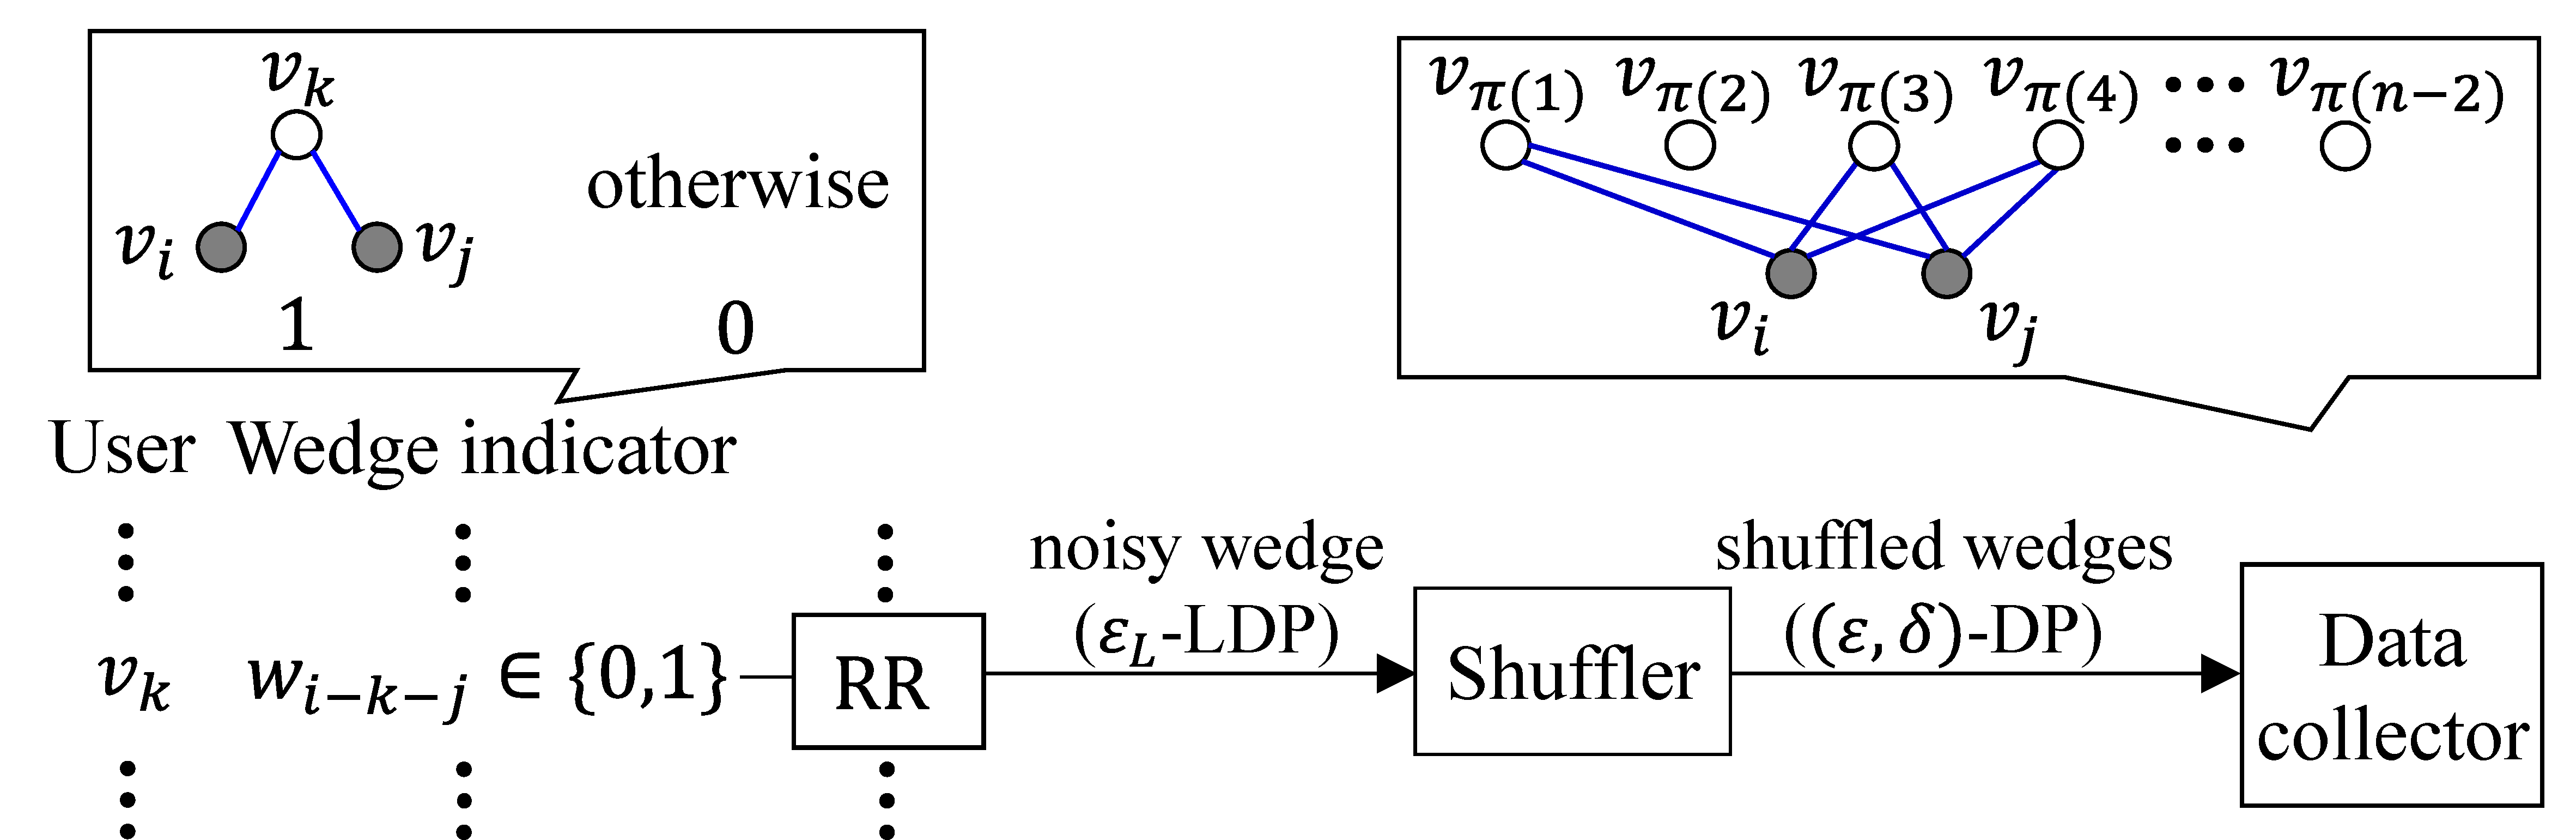
\includegraphics[width=0.99\linewidth]{fig/wedge_shuffle.pdf}
  
  \caption{Overview of our wedge shuffle algorithm with inputs $v_i$ and $v_j$. 
  %(marked with gray).
  }
  \label{chap3-fig:wedge_shuffle}
% \end{figure}
\vspace{2mm}
% \begin{figure}[t]
  \centering
  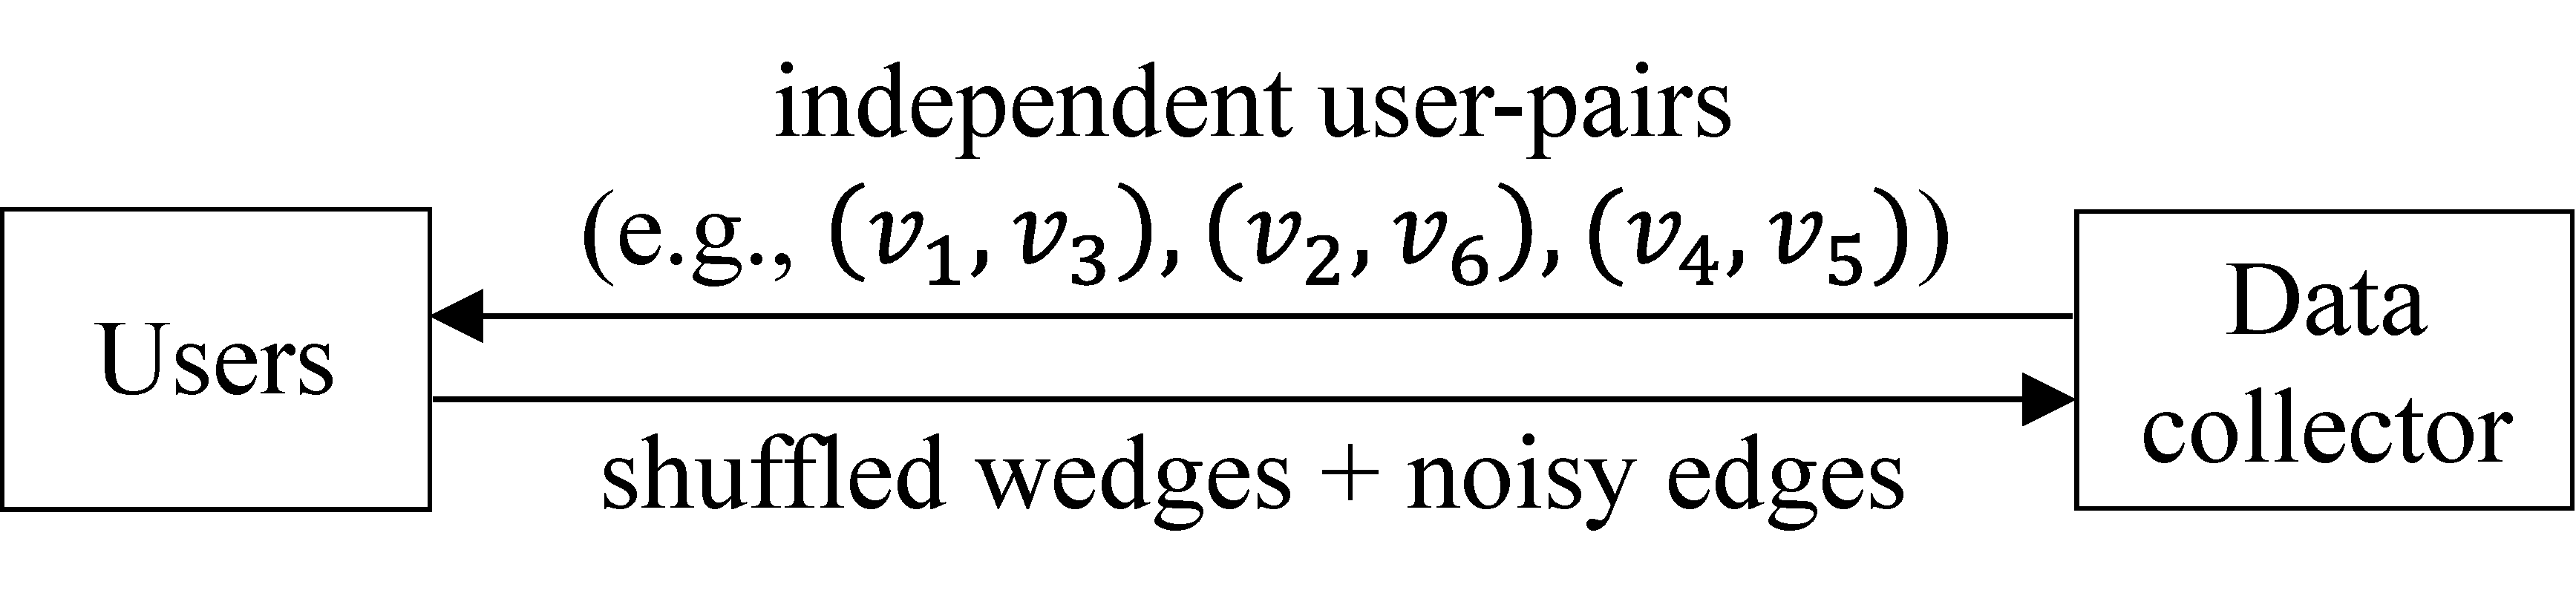
\includegraphics[width=0.7\linewidth]{fig/triangle_count.pdf}
  
  \caption{Overview of our triangle counting algorithm. 
  We use our wedge shuffle algorithm with each user-pair.
  %Independent pairs of nodes do share common nodes, e.g., $(v_1, v_3)$, $(v_2, v_6)$, $(v_4, v_5)$.
  }
  \label{chap3-fig:triangle_count}
\end{figure}

\smallskip
\noindent{\textbf{Shuffling Wedges.}}~~First, we propose a basic technique, which we call wedge shuffling, to enable privacy amplification of graph data by shuffling. 
% the application of shuffling to graph data. 
Specifically, we consider the problem of counting triangles including a specific user-pair $(v_i, v_j)$ 
% two specific nodes $v_i$ and $v_j$ 
and propose a wedge shuffle algorithm to accurately count them. 
Given $v_i$ and $v_j$, 
our wedge shuffle algorithm calculates a \textit{wedge indicator} $w_{i-k-j} \in \{0,1\}$, which 
takes $1$ if and only if a wedge (two-path) 
% from $v_i$ to $v_j$ 
$v_i$-$v_k$-$v_j$ 
exists, 
% indicates whether a two-hop path from $v_i$ to $v_j$ exists, 
for each of the remaining users $v_k$ ($k \ne i, j$). 
% of user $v_k$ ($k \ne i, j$), which indicates whether a two-hop path $v_i-v_k-v_j$ exists, rather than the entire neighbor lists. 
Then, it 
% uses the wedge indicator 
% , rather than the entire neighbor list, 
% as input data in the shuffle model. 
obfuscates the wedge indicators using $\epsilon_L$-RR and shuffles them to provide $(\epsilon, \delta)$-DP with $\epsilon \ll \epsilon_L$. 
Because the wedge indicator $w_{i-k-j}$ is one-dimensional, it can be sent with 
% large $\epsilon_L$ (i.e., small noise) 
small noise 
and small $\epsilon$, 
% small noise and small privacy budget, 
unlike the $n$-dimensional neighbor list. 
For example, when $n=10^5$, $\delta=10^{-8}$, and $\epsilon=1$, the value of $\epsilon_L$ in (\ref{chap3-eq:shuffle_epsilon_f}) and (\ref{chap3-eq:shuffle_epsilon}) is $\epsilon_L = 5.44$. 
In this case, $\epsilon_L$-RR rarely flips $w_{i-k-j}$ -- the flip probability is $0.0043$. 

\smallskip
\noindent{\textbf{Sending Local Edges.}}~~The shuffled wedge indicators tell us the number of common friends of $v_i$ and $v_j$. 
However, the data collector still cannot count triangles, because she does not know whether $v_i$ and $v_j$ are friends. 
Thus, our wedge shuffle algorithm sends \textit{local edges} between $v_i$ and $v_j$ to the data collector. 
Specifically, it 
obfuscates edge indicators $a_{i,j}$ and $a_{j,i}$ using $\epsilon$-RR and directly sends 
them 
to the data collector without shuffling\footnote{It is also possible to send the noisy edge indicators from users $v_i$ and $v_j$ to the data collector through the shuffler. In this case, the shuffler does not shuffle these data.}. 
Then, the data collector calculates an unbiased estimate of the triangle count from the noisy data. 
% from the shuffled wedge indicators and the noisy edge indicators. 
Because $\epsilon$ is small, a large amount of noise is added to the edge indicators. 
However, \textit{only one edge} is noisy (the other two have little noise) in any triangle the data collector sees. 
This brings us an advantage over the one-round local algorithms in which all three edges are noisy. 

\smallskip
\noindent{\textbf{Sampling Independent User-Pairs.}}~~Now, we turn our attention to the problem of counting triangles in the entire graph $G$. 
A naive solution to this problem is to use our wedge shuffling with all $\binom{n}{2}$ user-pairs as input. 
However, it results in very large $\epsilon$ and $\delta$ because it uses each element of the adjacency matrix $\bmA$ many times. 
To address this issue, 
% To accurately count them under DP, 
we propose a triangle counting algorithm that samples 
% independent edges (a.k.a. matching), which have no nodes in common. 
independent user-pairs, which share no common users. 
% and then uses the wedge shuffling algorithm for each sampled edge. 
The data collector sends the sampled user-pairs to users. 
Then, users apply our wedge shuffling algorithm with each user-pair 
% as input 
and send the results to the data collector. 
% Finally, the data collector calculates an unbiased estimate of the triangle count from the results. 
% This can be viewed as edge sampling \cite{Bera_KDD20,Eden_FOCS15,Wu_TKDE16} in triangle counting. 
% Edge sampling is known as an efficient sampling method that outperforms other sampling methods such as node sampling and triangle sampling \cite{Wu_TKDE16}. 
% Our triangle counting algorithm is also efficient and 
% In fact, 
Because our triangle algorithm uses each element of 
% the adjacency matrix 
$\bmA$ at most once, it provides $(\epsilon,\delta)$-element DP hence $(2\epsilon,2\delta)$-edge DP. 
In addition, our triangle algorithm reduces the time complexity from $O(n^3)$ to $O(n^2)$ by sampling user-pairs rather than using all user-pairs. 
% In addition, our wedge shuffle algorithm with a user-pair $(v_i,v_j)$ provides $(\epsilon,\delta)$-DP for each row in the $i$-th and $j$-th columns of the adjacency matrix $\bmA$, and our triangle algorithm samples independent user-pairs. 
% Thus, our algorithm provides $(\epsilon,\delta)$-element DP hence $(2\epsilon,2\delta)$-edge DP. 

We prove that the expected $l_2$ loss of our triangle counting algorithm is 
% $O(n^3 d_{max}^2)$. 
$O(n^3)$ when we ignore the factor of $d_{max}$. 
% when we regard $\epsilon$ and $\delta$ as constants. 
When we do not shuffle wedges, the 
% expected 
$l_2$ loss is 
% $O(n^5)$. 
$O(n^4)$. 
% This is much smaller than the existing one-round local algorithm with the same time complexity, whose $l_2$ loss is $O(n^5)$, as shown in Section~\ref{chap3-sub:upper}. 
In addition, the $l_2$ loss of the existing one-round local algorithm \cite{Imola_USENIX22} with the same time complexity is $O(n^5)$, as shown in 
Appendix~\ref{chap3-sec:upper}. 
% Section~\ref{chap3-sub:upper}. 
% Thus, our algorithm has a much smaller estimation error than the local algorithm. 
Thus, our wedge shuffling provides a dramatic improvement over the local algorithms. 

\smallskip
\noindent{\textbf{Variance Reduction.}}~~Although our wedge shuffling dramatically reduces the $l_2$ loss, the factor of $n^3$ is still large. 
Therefore, we propose a variance reduction technique that ignores sparse user-pairs, where either of the two users has a very small degree. 
Our basic idea is that the number of triangles including such a user-pair is very small 
% such user-pairs have a very small number of triangles 
and therefore can be approximated by $0$. 
By ignoring the sparse user-pairs, we can significantly reduce the variance at the cost of introducing a small bias. 
We prove that our variance reduction technique reduces the expected $l_2$ loss from $O(n^3)$ to $O(n^2)$ and makes accurate one-round triangle counting possible. 
% This enables us to accurately count triangles within one round. 

% \subsection{Triangle Counting Including a Specific Edge}
% \label{chap3-sub:triangle_edge}
\subsection{Wedge Shuffle}
\label{chap3-sub:wedge}
% Each user $v_k$ ($k \ne i, j$) calculates wedge information $w_{i-k-j} \in \{0,1\}$ that takes $1$ if there is a two-hop path $v_i-v_k-v_j$ and 0 otherwise. 
% Then $v_k$ obfuscates $w_{i-k-j}$ using $\epsilon_L$-RR and sends the noisy wedge to the shuffler. 
% The shuffler randomly shuffles the noisy wedges to provide $(\epsilon, \delta)$-DP with $\epsilon \ll \epsilon_L$ and sends them to the data collector. 
% In addition, users $v_i$ and $v_j$ obfuscate edge information $a_{i,j}$ and $a_{j,i}$, respectively, using $\epsilon$-RR and directly send them to the data collector. 

% \smallskip
\noindent{\textbf{Algorithm.}}~~We first 
%Consider the problem of counting triangles including a specific user-pair $(v_i,v_j)$. 
% To solve this problem, we 
propose a wedge shuffle algorithm, which estimates the number of triangles including a specific user-pair $(v_i,v_j)$. 
We denote this algorithm by \AlgWS{}. 

Algorithm~\ref{chap3-alg:wshuffle} shows \AlgWS{}. 
% This algorithm estimates the number of triangles including a specific user-pair $(v_i,v_j)$. 
Let $f_{i,j}^\triangle: \calG \rightarrow \nnints$ be a function that takes $G \in \calG$ as input and outputs the number $f_{i,j}^\triangle(G)$ of triangles including $(v_i,v_j)$ in $G$. 
Let $I_{-(i,j)}$ be the set of indices of users other than $v_i$ and $v_j$, i.e., $I_{-(i,j)} = [n]\setminus\{i,j\}$. 

\setlength{\algomargin}{5mm}
\begin{algorithm}[t]
  \SetAlgoLined
  \KwData{Adjacency matrix $\bmA \in \{0,1\}^{n \times n}$, 
    %Neighbor lists $\bma_1, \ldots, \bma_n \in \{0,1\}^n$, 
    %$\epsilon_L \in \nnreals$, $\delta \in [0,1]$, $\epsilon = f(n-2, \epsilon_L, \delta)$, 
    $\epsilon \in \nnreals$, $\delta \in [0,1]$, 
    user-pair $(v_i,v_j)$.
  }
  \KwResult{Estimate $\hf_{i,j}^\triangle(G)$ of the number $f_{i,j}^\triangle(G)$ of triangles including $(v_i,v_j)$.} 
  %of the count of triangles including $(v_i,v_j)$.}
  \tcc{Set-up}
  $I_{-(i,j)} \leftarrow [n]\setminus\{i,j\}$\;
  $\epsilon_L \leftarrow \texttt{LocalPrivacyBudget}(n,\epsilon,\delta)$\;
  \tcc{Users}
%   \For{$i=1$ \KwTo $n$}{
  \ForEach{$k \in I_{-(i,j)}$}{
    [$v_k$] $w_{i-k-j} \leftarrow a_{k,i} a_{k,j}$\;
    [$v_k$] $y_k \leftarrow \calR_{\epsilon_L}^W(x)(w_{i-k-j})$\;
    [$v_k$] Send $y_k$ to the shuffler\;
  }
  [$v_i$] $z_i \leftarrow \calR_{\epsilon}^W(x)(a_{i,j})$\;
  [$v_i$] Send $z_i$ to the data collector\;
  [$v_j$] $z_j \leftarrow \calR_{\epsilon}^W(x)(a_{j,i})$\;
  [$v_j$] Send $z_j$ to the data collector\;
  \tcc{Shuffler}
  [s] Sample a random permutation $\pi$ over $I_{-(i,j)}$\;
  [s] Send $\{y_{\pi(k)} | k \in I_{-(i,j)}\}$ to the data collector\;
  \tcc{Data collector}
  [d] $q_L \leftarrow \frac{e^{\epsilon_L}}{e^{\epsilon_L}+1}$; $q \leftarrow \frac{e^\epsilon}{e^\epsilon+1}$\;
  [d] $\hf_{i,j}^\triangle(G) \leftarrow \frac{(z_i+z_j-2(1-q))\sum_{k \in I_{-(i,j)}} (y_{\pi(k)} - (1-q_L))}{2(2q-1)(2q_L-1)}$\;
  \KwRet{$\hf_{i,j}^\triangle(G)$}
  \caption{Our wedge shuffle algorithm \AlgWS{}.
  [$v_i$], [s], [d] represent that the process is run by user $v_i$, the shuffler, and the data collector, respectively. 
  % Lines 1 and 2 are run by all parties. 
  }\label{chap3-alg:wshuffle}
\end{algorithm}

% Given $\epsilon$ and $\delta$, 
We first call the function \texttt{LocalPrivacyBudget}, which calculates a local privacy budget $\epsilon_L$ from $n$, $\epsilon$, and $\delta$ (line 2). 
Specifically, this function calculates $\epsilon_L$ 
such that $\epsilon$ is a closed-form upper bound (i.e., $\epsilon = f(n-2, \epsilon_L, \delta)$ in (\ref{chap3-eq:shuffle_epsilon_f})) or numerical upper bound in the shuffle model with $n-2$ users. 
% \cite{Feldman_FOCS21}. 
Given $\epsilon_L$, we can easily calculate the closed-form or numerical upper bound $\epsilon$ by (\ref{chap3-eq:shuffle_epsilon}) and the open source code in \cite{Feldman_FOCS21}\footnote{\url{https://github.com/apple/ml-shuffling-amplification}.}, respectively. 
Thus, we can also easily calculate $\epsilon_L$ from $\epsilon$ by calculating a lookup table for pairs $(\epsilon, \epsilon_L)$. 

Then, each user $v_k \in I_{-(i,j)}$ calculates a wedge indicator $w_{i-k-j} \in \{0,1\}$ from her neighbor list $\bma_k$ as follows: $w_{i-k-j} = a_{k,i} a_{k,j}$. 
User $v_k$ obfuscates $w_{i-k-j}$ using $\epsilon_L$-RR $\calR_{\epsilon_L}^W$ and sends the result $y_k = \calR_{\epsilon_L}^W(w_{i-k-j})$ to the shuffler (lines 4-6). 
Meanwhile, user $v_i$ obfuscates $a_{i,j}$ using $\epsilon$-RR $\calR_{\epsilon}^W$ and sends the result $z_i = \calR_{\epsilon}^W(a_{i,j})$ to the data collector\footnotemark[1] (lines 8-9). 
Similarly, user $v_j$ sends $z_j = \calR_{\epsilon}^W(a_{j,i})$ to the data collector (lines 10-11). 

The shuffler samples a uniform random permutation $\pi$ over $I_{-(i,j)}$ and shuffles the wedge indicators based on $\pi$. 
Then, the shuffler sends the shuffled wedge indicators $\{y_{\pi(k)} | k \in I_{-(i,j)}\}$ to the data collector (lines 12-13). 

% After receiving $\{y_{\pi(k)} | k \in I_{-(i,j)}\}$, $z_i$, and $z_j$, 
Finally, the data collector estimates $f_{i,j}^\triangle(G)$ from $\{y_{\pi(k)} | k \in I_{-(i,j)}\}$, $z_i$, $z_j$. 
Specifically, let $\hf_{i,j}^\triangle(G) \in \reals$ be an estimate of $f_{i,j}^\triangle(G)$. 
The data collector calculates $\hf_{i,j}^\triangle(G)$ as follows: 
\begin{align}
    \hf_{i,j}^\triangle(G) = \frac{(z_i+z_j-2(1-q))\sum_{k \in I_{-(i,j)}} (y_{\pi(k)} - (1-q_L))}{2(2q-1)(2q_L-1)},
    \label{chap3-eq:hfij_triangle}
\end{align}
where $q_L = \frac{e^{\epsilon_L}}{e^{\epsilon_L}+1}$ and $q = \frac{e^\epsilon}{e^\epsilon+1}$ (lines 14-15). 
As we prove later, $\hf_{i,j}^\triangle(G)$ in (\ref{chap3-eq:hfij_triangle}) is an unbiased estimate of $f_{i,j}^\triangle(G)$. 

\smallskip
\noindent{\textbf{Theoretical Properties.}}~~Below, we show some theoretical properties of \AlgWS{}. 
First, we prove that \AlgWS{} provides DP: 
\begin{theorem}
\label{chap3-thm:DP_I}
\AlgWS{} provides $(\epsilon, \delta)$-element DP and $(2\epsilon, 2\delta)$-edge DP. 
\end{theorem}
Intuitively, Theorem~\ref{chap3-thm:DP_I} comes from the fact that \AlgWS{} uses only the $i$-th and $j$-th columns of the adjacency matrix $\bmA$ and protects each element with $(\epsilon,\delta)$-DP. 
See Appendix~\ref{chap3-sec:triangle_proof} for details. 

Next, we prove that the estimate $\hf_{i,j}^\triangle(G)$ of \AlgWS{} is unbiased: 
% of $f_{i,j}^\triangle(G)$: 
\begin{theorem}
\label{chap3-thm:unbiased_I}
In \AlgWS{}, $\E[\hf_{i,j}^\triangle(G)] = f_{i,j}^\triangle(G)$. 
% \AlgWS{} provides an unbiased estimate, i.e., 
% \begin{align*}
% \E[\hf_{i,j}^\triangle(G)] = f_{i,j}^\triangle(G).
% \end{align*}
\end{theorem}

Finally, we show the expected $l_2$ loss ($=$ variance) of \AlgWS{}. 
% $\hf_{i,j}^\triangle(G)$. 
Recall that in the shuffle model, $\epsilon_L = \Theta(\log n)$ when we treat $\epsilon$ and $\delta$ as constants. 
%see Section~\ref{chap3-sub:shuffle}
We show 
% the expected $l_2$ losses for a general case and the case where $\epsilon_L = \Theta(\log n)$: 
the $l_2$ loss for a general case and for the shuffle model:
\begin{theorem}
\label{chap3-thm:l2-loss_I}
\AlgWS{} provides the following utility guarantee: 
% In \AlgWS{}, 
\begin{align}
& l_2^2(f_{i,j}^\triangle(G), \hf_{i,j}^\triangle(G)) = \V[\hf_{i,j}^\triangle(G)] \nonumber\\ 
& \leq \frac{n q_L(1-q_L) + q(1-q)(2q_L-1)^2 (\sum_{k \in I_{-(i,j)}}w_{i-k-j})^2}{(2q-1)^2(2q_L-1)^2}.
\label{chap3-eq:l2_I_general}
\end{align}
When $\epsilon_L = \Theta(\log n)$, 
% we have 
\begin{align}
& l_2^2(f_{i,j}^\triangle(G), \hf_{i,j}^\triangle(G)) = \V[\hf_{i,j}^\triangle(G)] \nonumber\\ 
& \leq \frac{q(1-q)(2q_L-1)^2 (\sum_{k \in I_{-(i,j)}}w_{i-k-j})^2}{(2q-1)^2(2q_L-1)^2} + O(1).
\label{chap3-eq:l2_I_shuffle}
\end{align}
\end{theorem}
% Theorem~\ref{chap3-thm:l2-loss_I} states that 
By (\ref{chap3-eq:l2_I_general}), if we do not use the shuffling technique (i.e., $\epsilon_L = \epsilon$), the $l_2$ loss can be expressed as $l_2^2(f_{i,j}^\triangle(G), \hf_{i,j}^\triangle(G)) = O(n + d_{max}^2)$. 
In contrast, the $l_2$ loss in (\ref{chap3-eq:l2_I_shuffle}) is $l_2^2(f_{i,j}^\triangle(G), \hf_{i,j}^\triangle(G)) = O(d_{max}^2)$ because there are at most $d_{max}$ wedges from $v_i$ to $v_j$, i.e., $\sum_{k \in I_{-(i,j)}}w_{i-k-j} = O(d_{max})$. 
% This means that the $l_2$ loss is reduced from $O(n + d_{max}^2)$ to $O(d_{max}^2)$ by shuffling wedges. 
This means that wedge shuffling reduces the $l_2$ loss from $O(n + d_{max}^2)$ to $O(d_{max}^2)$, which is significant when $d_{max} \ll n$. 

% \subsection{Triangle Counting Based on Wedge Shuffle}
\subsection{Wedge Shuffle-Based Triangle Counting}
\label{chap3-sub:triangle}
\noindent{\textbf{Algorithm.}}~~Our wedge shuffle algorithm \AlgWS{} estimates the number of triangles including a specific user-pair $(v_i,v_j)$. 
Based on this, we propose an algorithm that 
% estimates the triangle count $f^\triangle(G)$ 
counts triangles in the entire graph $G$. 
We denote this algorithm by \AlgWSTri{}. 

Algorithm~\ref{chap3-alg:wshuffle_triangle} shows \AlgWSTri{}. 
First, the data collector samples independent user-pairs, which share no common users. 
Specifically, it calls the function \texttt{RandomPermutation}, which samples a uniform random permutation $\sigma$ over $[n]$ (line 1). 
Then, it samples independent user-pairs as 
$(v_{\sigma(1)}, v_{\sigma(2)}), (v_{\sigma(3)}, v_{\sigma(4)}), \ldots, (v_{\sigma(2t-1)}, v_{\sigma(2t)})$, where $t \in [\lfloor \frac{n}{2} \rfloor]$. 
The parameter $t$ represents the number of user-pairs and controls the trade-off between the $l_2$ loss and the time complexity; 
when $t = \lfloor \frac{n}{2} \rfloor$, the $l_2$ loss is minimized and the time complexity is maximized. 
The data collector sends the sampled user-pairs to users (line 2).

\setlength{\algomargin}{5mm}
\begin{algorithm}[t]
  \SetAlgoLined
  \KwData{Adjacency matrix $\bmA \in \{0,1\}^{n \times n}$, $\epsilon \in \nnreals$, $\delta \in [0,1]$, $t \in [\lfloor \frac{n}{2} \rfloor]$.
  }
  \KwResult{Estimate $\hf^\triangle(G)$ of $f^\triangle(G)$.} 
%   \tcc{Data collector}
  [d] $\sigma \leftarrow$\texttt{RandomPermutation}$(n)$\;
  [d] Send $(v_{\sigma(1)}, v_{\sigma(2)}), \ldots, (v_{\sigma(2t-1)}, v_{\sigma(2t)})$ to users\;
%  \ForEach{$i \in \{1, 3, \ldots, 2t-1\}$}{
%    [$d$] Send $(\sigma(i), \sigma(i+1))$ to users\;
%  }
%   \tcc{Users, shuffler, and data collector}
  \ForEach{$i \in \{1, 3, \ldots, 2t-1\}$}{
    $\hf_{\sigma(i), \sigma(i+1)}^\triangle(G) \leftarrow$ \AlgWS{}$(\bmA, \epsilon, \delta, (v_{\sigma(i)}, v_{\sigma(i+1)}))$\;
  }
%   \tcc{Data collector}
  [d] $\hf^\triangle(G) \leftarrow \frac{n(n-1)}{6t} \sum_{i=1, 3, \ldots, 2t-1} \hf_{\sigma(i),\sigma(i+1)}^\triangle(G)$\;
  \KwRet{$\hf^\triangle(G)$}
  \caption{Our wedge shuffle-based triangle counting algorithm \AlgWSTri{}.
  [d] represents that the process is run by the data collector. 
  \AlgWS{} is shown in Algorithm~\ref{chap3-alg:wshuffle}. 
  }\label{chap3-alg:wshuffle_triangle}
\end{algorithm}

Then, we run our wedge algorithm \AlgWS{} in Algorithm~\ref{chap3-alg:wshuffle} with each sampled user-pair as input (lines 3-5). 
Finally, the data collector estimates the triangle count $f^\triangle(G)$ as follows: 
\begin{align}
    \hf^\triangle(G) = \textstyle{\frac{n(n-1)}{6t} \sum_{i=1, 3, \ldots, 2t-1} \hf_{\sigma(i),\sigma(i+1)}^\triangle(G)} 
   \label{chap3-eq:hf_triangle_II}
\end{align}
(line 6). Later, we prove that $\hf^\triangle(G)$ in (\ref{chap3-eq:hf_triangle_II}) is unbiased. 

\smallskip
\noindent{\textbf{Theoretical Properties.}}~~We now prove that our triangle counting algorithm \AlgWSTri{} provides DP: 
% Below, we show the privacy and utility of \AlgWSTri{}. 
% We first prove that \AlgWSTri{} provides DP: 
\begin{theorem}
\label{chap3-thm:DP_II}
\AlgWSTri{} provides $(\epsilon, \delta)$-element DP and $(2\epsilon, 2\delta)$-edge DP. 
\end{theorem}
Theorem~\ref{chap3-thm:DP_II} comes from the fact that 
\AlgWS{} with a user-pair $(v_i,v_j)$ provides $(\epsilon,\delta)$-DP for each element in the $i$-th and $j$-th columns of the adjacency matrix $\bmA$ and that \AlgWSTri{} samples independent user-pairs, i.e., it uses each element of $\bmA$ at most once. 
% and protect each element with $(\epsilon,\delta)$-DP. 

Note that running \AlgWS{} with all $\binom{n}{2}$ user-pairs requires a very large privacy budget --  
% By composition, 
it provides $((n-1) \epsilon, (n-1) \delta)$-DP, as it uses each element of $\bmA$ at most $n-1$ times. 
The privacy budget is very large even using the advanced composition \cite{DP,Kairouz_ICML15}. 
We avoid this issue by sampling user-pairs that share no common users. 

We also prove that 
% the estimate of \AlgWSTri{} is unbiased: 
\AlgWSTri{} provides an unbiased estimate: 
% Next, we show the utility of \AlgWSTri{}: 
\begin{theorem}
\label{chap3-thm:unbiased_II}
In \AlgWSTri{}, $\E[\hf^\triangle(G)] = f^\triangle(G)$. 
% \AlgWSTri{} provides an unbiased estimate, i.e., 
% \begin{align*}
% \E[\hf^\triangle(G)] = f^\triangle(G).
% \end{align*}
\end{theorem}

Next, we analyze the expected $l_2$ loss ($=$ variance) of \AlgWSTri{}. 
This analysis is complicated because \AlgWSTri{} samples each user-pair \textit{without replacement}. 
In this case, the sampled user-pairs are not independent. 
However, we can prove that 
$t$ estimates in (\ref{chap3-eq:hf_triangle_II}) are negatively correlated with each other (Lemma~\ref{chap3-lem:cov} in Appendix~\ref{chap3-sub:l2-loss_II_proof}). 
%the covariance of two estimates $\hf_{\sigma(i),\sigma(i+1)}^\triangle(G)$ and $\hf_{\sigma(j),\sigma(j+1)}^\triangle(G)$ in (\ref{chap3-eq:hf_triangle_II}) 
Thus, the variance of the sum of $t$ estimates 
%$\sum_{i=1, 3, \ldots, 2t-1} \hf_{\sigma(i),\sigma(i+1)}^\triangle(G)$ 
in (\ref{chap3-eq:hf_triangle_II}) is upper bounded by the sum of their variances, each of which is given by Theorem~\ref{chap3-thm:l2-loss_I}. 
This brings us the following result: 

\begin{theorem}
\label{chap3-thm:l2-loss_II}
\AlgWSTri{} provides the following utility guarantee:
\begin{align}
& l_2^2(f^\triangle(G), \hf^\triangle(G)) = \V[\hf^\triangle(G)] \nonumber\\ 
% & \leq \frac{n^2(n-1)^2}{36t^2} \left(g(t, \sigma, G) + \frac{t d_{max}^3}{n-1}\right), \label{chap3-eq:thm:l2_II}
& \leq \frac{n^2(n-1)^2}{36t^2} \left(\E_\sigma \left[ \sum_{i=1, 3, \ldots, 2t-1} 
g(\sigma(i),\sigma(i+1)) \right] + \frac{t d_{max}^3}{n-1}\right), \label{chap3-eq:thm:l2_II}
% & \leq \frac{n^2(n-1)^2}{36t^2} \left(\E_\sigma \left[ \sum_{i=1, 3, \ldots, 2t-1} 
% l_2^2(f_{\sigma(i),\sigma(i+1)}^\triangle(G), \hf_{\sigma(i),\sigma(i+1)}^\triangle(G)) \right]\right. \nonumber\\
% &\hspace{20mm} \left. + \frac{t d_{max}^3}{n-1}\right), \label{chap3-eq:thm:l2_II}
\end{align}
where $\E_\sigma$ is the expectation over the permutation $\sigma$ and 
\begin{align}
% g(t, \sigma, G) = \E_\sigma \left[ \sum_{i=1, 3, \ldots, 2t-1} l_2^2(f_{\sigma(i),\sigma(i+1)}^\triangle(G), \hf_{\sigma(i),\sigma(i+1)}^\triangle(G)) \right],
g(\sigma(i),\sigma(i+1)) = l_2^2(f_{\sigma(i),\sigma(i+1)}^\triangle(G), \hf_{\sigma(i),\sigma(i+1)}^\triangle(G)) 
\label{chap3-eq:thm:g}
\end{align}
% where 
% $l_2^2(f_{\sigma(i),\sigma(i+1)}^\triangle(G), \hf_{\sigma(i),\sigma(i+1)}^\triangle(G))$ 
is the expected $l_2$ loss of \AlgWS{} with input $(v_{\sigma(i)},v_{\sigma(i+1)})$ (see Theorem~\ref{chap3-thm:l2-loss_I}). 
% and $\E_\sigma$ is the expectation over the permutation $\sigma$. 
\end{theorem}
% Theorem~\ref{chap3-thm:unbiased_II} states that the estimate of \AlgWSTri{} is unbiased. 

The first and second terms in (\ref{chap3-eq:thm:l2_II}) are caused by 
% the randomness in 
Warner's RR for local edges and the sampling of independent user-pairs, respectively. 
In other words, the $l_2$ loss of \AlgWSTri{} can be decomposed into two factors: the RR for local edges and user-pair sampling. 

For example, assume that $t = \lfloor \frac{n}{2} \rfloor$. 
When we do not shuffle wedges (i.e., $\epsilon_L = \epsilon$), the $l_2$ loss in (\ref{chap3-eq:thm:l2_II}) is $O(n^4 + n^3 d_{max}^2 + n^2 d_{max}^3)$. 
When we shuffle wedges, the $l_2$ loss is $O(n^3 d_{max}^2 + n^2 d_{max}^3)$. 
Thus, when we ignore the factor of $d_{max}$, our wedge shuffle technique reduces the $l_2$ loss from $O(n^4)$ to $O(n^3)$ in triangle counting. 
The factor of $n^3$ is caused by the RR for local edges. 
This is intuitive because a large amount of noise is added to the local edges. 

Finally, we analyze the time complexity of \AlgWSTri{}. 
The time complexity of running \AlgWS{} with all $\binom{n}{2}$ user-pairs is $O(n^3)$, as there are $O(n^2)$ user-pairs in total and \AlgWS{} requires the time complexity of $O(n)$. 
In contrast, the time complexity of \AlgWSTri{} is $O(n^2)$ because it samples $O(n)$ user-pairs. 
Thus, \AlgWSTri{} reduces the time complexity from $O(n^3)$ to $O(n^2)$ by user-pair sampling. 
We can further reduce the time complexity by setting the number $t$ of sampled user-pairs small, i.e., $t \ll \lfloor \frac{n}{2} \rfloor$. 
However, it comes at the cost of increasing the $l_2$ loss. 

% \subsection{Variance Reduction Based on Ignoring Sparse User-Pairs}
\subsection{Variance Reduction}
\label{chap3-sub:var_red}
\noindent{\textbf{Algorithm.}}~~Our 
% wedge shuffle-based 
triangle counting algorithm \AlgWSTri{} achieves the $l_2$ loss of $O(n^3)$ when we ignore the factor of $d_{max}$. 
However, the factor of $n^3$ is still large because the square of the true count $f^\triangle(G)$ is $O(n^2)$. 
To provide a small relative error, we should reduce the $l_2$ loss of \AlgWSTri{} from $O(n^3)$ to at most $O(n^2)$. 
To this end, we propose a variance reduction technique that ignores sparse user-pairs. 
We denote our triangle counting algorithm with the variance reduction technique by \AlgWSTriVR{}. 

% Let $d_{i,j} = \min\{d_i, d_j\}$ be the minimum degree of users $v_i$ and $v_j$. 
As explained in Section~\ref{chap3-sub:triangle}, the factor of $n^3$ is caused by the RR for local edges. 
However, most user-pairs $v_i$ and $v_j$ have a very small minimum degree 
% $d_{i,j} \ll d_{max}$, 
$\min\{d_i, d_j\} \ll d_{max}$, 
and there is no edge $(v_i, v_j)$ between them in almost all cases. 
In addition, even if there is an edge $(v_i, v_j)$, the number of triangles including the sparse user-pair is very small 
% (at most $d_{i,j}-1$) 
(at most $\min\{d_i, d_j\}$) 
and can be approximated by $0$. 
% Thus, 
% we can approximate the number of triangles including the sparse user-pair by $0$. 
By ignoring such sparse user-pairs, we can dramatically reduce the variance of the RR for local edges at the cost of a small bias. 
This is an intuition behind our variance reduction technique. 

% Specifically, we consider the following improvement of \AlgWSTri{}. 
% Let $d_{i,j} = \min\{d_i, d_j\}$ be the minimum degree of users $v_i$ and $v_j$. 
% Below, we assume that the data collector knows each user $v_i$'s degree $d_i$ for ease of explanation. 
% Note that $d_i$ can leak the information about edges of $v_i$. 
% Thus, we explain how to privately estimate $d_i$ with edge DP within one-round at the end of Section~\ref{chap3-sub:var_red}. 
Algorithm~\ref{chap3-alg:wshuffle_triangle_vr} shows \AlgWSTriVR{}. 
This algorithm detects sparse user-pairs based on the degree information. 
However, user $v_i$'s degree $d_i$ can leak the information about edges of $v_i$. 
Thus, \AlgWSTriVR{} calculates a differentially private estimate of $d_i$ within one-round. 

\setlength{\algomargin}{5mm}
\begin{algorithm}[t]
  \SetAlgoLined
  \KwData{Adjacency matrix $\bmA \in \{0,1\}^{n \times n}$, $\epsilon_1, \epsilon_2 \in \nnreals$, $\delta \in [0,1]$, $t \in [\lfloor \frac{n}{2} \rfloor]$, $c \in \nnreals$.
  }
  \KwResult{Estimate $\hf^\triangle(G)$ of $f^\triangle(G)$.} 
%   \tcc{Data collector}
  [d] $\sigma \leftarrow$\texttt{RandomPermutation}$(n)$\;
  [d] Send $(v_{\sigma(1)}, v_{\sigma(2)}), \ldots, (v_{\sigma(2t-1)}, v_{\sigma(2t)})$ to users\;
%   \tcc{Users, shuffler, and data collector}
  \ForEach{$i \in \{1, 3, \ldots, 2t-1\}$}{
    $\hf_{\sigma(i), \sigma(i+1)}^\triangle(G) \leftarrow$ \AlgWS{}$(\bmA, \epsilon_2, \delta, (v_{\sigma(i)}, v_{\sigma(i+1)}))$\;
  }
%   \tcc{Users}
  \For{$i=1$ \KwTo $n$}{
    [$v_i$] $\td_i \leftarrow d_i + \Lap(\frac{1}{\epsilon_1})$\;
    [$v_i$] Send $\td_i$ to the data collector\;
  }
%   \tcc{Data collector}
%   [d] $d_{th} \leftarrow \frac{c}{n} \sum_{i=1}^n \td_i$\;
  [d] $\td_{avg} \leftarrow \frac{1}{n} \sum_{i=1}^n \td_i$; $d_{th} \leftarrow c \td_{avg}$\;
  [d] $D \leftarrow \{i | i = 1, 3, \ldots, 2t-1, 
  \min\{\td_{\sigma(i)}, \td_{\sigma(i+1)}\} > d_{th}\}$\;
  [d] $\hf^\triangle(G) \leftarrow \frac{n(n-1)}{6t} \sum_{i \in D} \hf_{\sigma(i),\sigma(i+1)}^\triangle(G)$\;
  \KwRet{$\hf^\triangle(G)$}
  \caption{Our triangle counting algorithm with variance reduction \AlgWSTriVR{}.
  [$v_i$] and [d] represent that the process is run by user $v_i$ and the data collector, respectively. 
  \AlgWS{} is shown in Algorithm~\ref{chap3-alg:wshuffle}. 
  }\label{chap3-alg:wshuffle_triangle_vr}
\end{algorithm}

Specifically, \AlgWSTriVR{} uses two privacy budgets: $\epsilon_1, \epsilon_2 \in \nnints$. 
The first budget $\epsilon_1$ is for privately estimating $d_i$, whereas the second budget $\epsilon_2$ is for wedge shuffling. 
Lines 1 to 5 in Algorithm~\ref{chap3-alg:wshuffle_triangle_vr} are the same as those in Algorithm~\ref{chap3-alg:wshuffle_triangle}, except that Algorithm~\ref{chap3-alg:wshuffle_triangle_vr} uses $\epsilon_2$ rather than $\epsilon$. 
After these processes, each user $v_i$ adds the Laplacian noise $\Lap(\frac{1}{\epsilon_1})$ with mean $0$ and scale $\frac{1}{\epsilon_1}$ to her degree $d_i$ and sends the noisy degree $\td_i$ ($= d_i + \Lap(\frac{1}{\epsilon_1})$) to the data collector (lines 6-9). 
% Since adding or removing one element changes $d_i$ by at most $1$ 

Then, the data collector estimates the average degree $d_{avg}$ as $\td_{avg} = \frac{1}{n}\sum_{i=1}^n \td_i$ and sets a threshold $d_{th}$ of the minimum degree to $d_{th} = c \td_{avg}$, where $c \in \nnreals$ is a small positive number, e.g., $c=1$ or $2$ (line 10). 
% (line 10). 
%$c \in \nnints$ times the private estimate $\frac{1}{n} \sum_{i=1}^n \td_i$ of $d_{avg}$ (line 10). 
Finally, the data collector estimates $f^\triangle(G)$ as follows: 
\begin{align}
    \hf^\triangle(G) = \textstyle{\frac{n(n-1)}{6t} \sum_{i \in D} \hf_{\sigma(i),\sigma(i+1)}^\triangle(G)}, 
   \label{chap3-eq:hf_triangle_II_ast}
\end{align}
where 
\begin{align*}
D = \{i | i = 1, 3, \ldots, 2t-1, 
  \min\{\td_{\sigma(i)}, \td_{\sigma(i+1)}\} > d_{th}\}
\end{align*}
(lines 11-12). 
The difference between (\ref{chap3-eq:hf_triangle_II}) and (\ref{chap3-eq:hf_triangle_II_ast}) is that (\ref{chap3-eq:hf_triangle_II_ast}) ignores sparse user-pairs $v_{\sigma(i)}$ and $v_{\sigma(i+1)}$ such that $\min\{\td_{\sigma(i)}, \td_{\sigma(i+1)}\} \leq d_{th}$. 
Because $d_{avg} \ll d_{max}$ in practice,  
$\min\{\td_{\sigma(i)}, \td_{\sigma(i+1)}\} \ll d_{max}$ holds for small $c$. 

The parameter $c$ controls the trade-off between the bias and variance of the estimate $\hf^\triangle(G)$. 
The larger $c$ is, the more user-pairs are ignored. 
Thus, as $c$ increases, the bias is increased and the variance is reduced. 
% Although the optimization of $c$ is challenging and is left for future work, 
In practice, $c=1$ or $2$ results in a small $l_2$ error % for the following reasons. 
% First, the bias is small in this case because $c d_{avg} \ll d_{max}$. 
% Second, 
% Note that 
because most real graphs are scale-free networks that have a power-law degree distribution \cite{NetworkScience}. 
% where 
In the scale-free networks, most users' degree are smaller than the average degree $d_{avg}$. 
For example, in the Barab\'{a}si-Albert graph model \cite{NetworkScience,Hagberg_SciPy08}, 
most users' degrees are $\frac{d_{avg}}{2}$. 
% with parameter (number of edges per node) $m$, the average degree is $d_{avg} = 2m$ and most users' degrees are $m$. 
Thus, if we set 
% $c \geq 1$, 
$c=1$ or $2$, 
% (e.g., $c=1$ or $2$), 
then most user-pairs are ignored (i.e., $|D| \ll t$), which leads to a significant reduction of the variance at the cost of a small bias. 
In our experiments, we set $c=1$. 

\smallskip
\noindent{\textbf{Theoretical Properties.}}~~\AlgWSTriVR{} provides the following privacy guarantee: 

\begin{theorem}
\label{chap3-thm:DP_II_ast}
\AlgWSTri{} provides $(\epsilon_1 + \epsilon_2, \delta)$-element DP and $(2(\epsilon_1 + \epsilon_2), 2\delta)$-edge DP. 
\end{theorem}

Theorem~\ref{chap3-thm:DP_II_ast} holds because \AlgWSTri{} provides $\epsilon_1$-element DP for degrees and $(\epsilon_2, \delta)$-element DP for wedges and edges. 

Next, we show the variance of \AlgWSTriVR{}:

\begin{theorem}
\label{chap3-thm:var_II_ast}
\AlgWSTriVR{} provides the following variance guarantee:
\begin{align}
& \V[\hf^\triangle(G)] \nonumber\\ 
& \leq \frac{n^2(n-1)^2}{36t^2} \left(\E_\sigma \left[ \sum_{i \in D} 
g(\sigma(i),\sigma(i+1)) \right] + \frac{t d_{max}^3}{n-1}\right), \label{chap3-eq:thm:l2_II_ast}
% & \leq \frac{n^2(n-1)^2}{36t^2} \left(\E_\sigma \left[ \sum_{i \in D} 
% l_2^2(f_{\sigma(i),\sigma(i+1)}^\triangle(G), \hf_{\sigma(i),\sigma(i+1)}^\triangle(G)) \right]\right. \nonumber\\
% &\hspace{20mm} \left. + \frac{t d_{max}^3}{n-1}\right). \label{chap3-eq:thm:l2_II_ast}
\end{align}
where $g(\sigma(i),\sigma(i+1))$ is given by (\ref{chap3-eq:thm:g}). 
% where $l_2^2(f_{\sigma(i),\sigma(i+1)}^\triangle(G), \hf_{\sigma(i),\sigma(i+1)}^\triangle(G))$ is the expected $l_2$ loss of \AlgWS{} with input $(v_{\sigma(i)},v_{\sigma(i+1)})$ (see Theorem~\ref{chap3-thm:l2-loss_I}) and $\E_\sigma$ is the expectation over the permutation $\sigma$. 
\end{theorem}
By (\ref{chap3-eq:thm:l2_II}) and (\ref{chap3-eq:thm:l2_II_ast}), our variance reduction technique dramatically reduces the variance when $|D| \ll t$. 
For example, when we shuffle wedges, the variance is $O(n^2|D|d_{max}^2 + n^2 d_{max}^3)$. 
Thus, we ignore the factor of $d_{max}$ and $|D|$ (both of which are much smaller than $n$), our technique reduces the variance from $O(n^3)$ to $O(n^2)$. 

Finally, we analyze the bias of \AlgWSTriVR{}. 
For simplicity, we assume that we do not add the Laplacian noise to $d_i$, i.e., $\td_i = d_i$. 
% In other words, we assume that each user $v_i$'s degree $d_i$ is public. 
This assumption is fine because 
$\Lap(\frac{1}{\epsilon_1})$ is very small in practice -- we show that adding $\Lap(\frac{1}{\epsilon_1})$ hardly affects the estimation error in our experiments. 
Under this assumption, we show the bias: 

\begin{theorem}
\label{chap3-thm:bias_II_ast}
Let $Bias[\hf^\triangle(G)]$ be the bias of $\hf^\triangle(G)$. 
\AlgWSTriVR{} ($\td_i = d_i$ for $i\in[n]$) 
% without the Laplacian noise 
provides the following bias guarantees:
\begin{align}
    Bias[\hf^\triangle(G)]^2 
    = (\E[\hf^\triangle(G)] - f^\triangle(G))^2 
    \leq \frac{n^2 d_{th}^4}{9}. 
    \label{chap3-eq:thm:bias_II_ast}
\end{align}
\end{theorem}

When $c$ is small (e.g., $c=1$ or $2$), $d_{th} = c d_{avg} \ll d_{max}$. 
Thus, the squared bias can be expressed as $O(n^2)$ by ignoring the factor of $d_{th}$. 
Because the expected $l_2$ loss is the summation of the squared bias and the variance, it can also be expressed as $O(n^2)$. 

\subsection{Summary}
\label{chap3-sub:summary}


\begin{table}[t]
  \centering
%   \begin{tabular}{|l|c|c|}
%     \hline
%     Algorithm & $l_2$ loss & Time complexity \\ \hline
%     \AlgWSTri{} & $O(n^3 d_{max}^2)$ & $O(n^2)$ \\ \hline
%     \AlgWSTriVR{}{} & $O(n^2 d_{max}^2 + n^2 d_{th}^4)$ & $O(n^2)$ \\ \hline
%     \AlgWLTri{} & $O(n^4 + n^3 d_{max}^2)$ & $O(n^2)$ \\ \hline
%     \AlgARRTri{} & $O(n^5)$ & $O(n^2)$ \\ \hline
%     \AlgRRTri{} & $O(n^4)$ & $O(n^3)$ \\ \hline
%   \end{tabular}
  \begin{tabular}{|l|c|c|c|c|}
    \hline
    Algorithm & Model & Variance & Bias$^2$ & Time \\ \hline
    \AlgWSTri{} & shuffle & $O(n^3 d_{max}^2)$ & $0$ & $O(n^2)$ \\ \hline
    \AlgWSTriVR{}{} & shuffle & $O(n^2 d_{max}^2)$ & $O(n^2 d_{th}^4)$ & $O(n^2)$ \\ \hline
    \AlgWLTri{} \cite{Imola_USENIX22} & local & $O(n^4 + n^3 d_{max}^2)$ & $0$ & $O(n^2)$ \\ \hline
    \AlgARRTri{} \cite{Imola_USENIX22} & local & $O(n^5)$ & $0$ & $O(n^2)$ \\ \hline
    \AlgRRTri{} \cite{Imola_USENIX21} & local & $O(n^4)$ & $0$ & $O(n^3)$ \\ \hline
  \end{tabular}
  \caption{Performance guarantees of one-round triangle counting algorithms providing edge DP. 
  ``Time'' represents the time complexity. 
  }
  \label{chap3-tab:upper_bounds}
\end{table}

Table~\ref{chap3-tab:upper_bounds} summarizes the performance guarantees of one-round triangle counting algorithms providing edge DP. 
Here, we show \AlgARRTri{} \cite{Imola_USENIX22} and \AlgRRTri{} \cite{Imola_USENIX21} as existing one-round local algorithms. 
We do not show the one-round local algorithms in \cite{Ye_ICDE20,Ye_TKDE21} for two reasons: (i) it is reported in \cite{Imola_USENIX22} that they are outperformed by \AlgRRTri{}; (ii) their upper-bounds on the variance and bias are unclear. 

Table~\ref{chap3-tab:upper_bounds} shows that our \AlgWSTriVR{} significantly outperforms the existing local algorithms. 
We also show this through experiments. 

% \subsection{Lower Bounds for Local Algorithms}
% \label{chap3-sub:two-rounds}
% TBD

% \subsection{Algorithm}
% \label{chap3-sub:triangle_algorithm}
% TBD

% \subsection{Theoretical Analysis}
% \label{chap3-sub:triangle_theoretical}
% TBD

% \subsection{4-Cycle Counting}
% \label{chap3-sub:4-cycle}
% TBD